\section{Architecture}
\subsection{Assessing Contribution Quality}
\begin{frame}
    \tikz[overlay, remember picture,
      shift=(current page.south west),
      x=(current page.south east),
      y=(current page.north west)
    ]{
        % Show the optional help grid lines 
        %\draw[step=.1, opacity=0.3, thick, red] (0,0) grid (1,1);
      
        \node[anchor=south east] at (1,0) {
            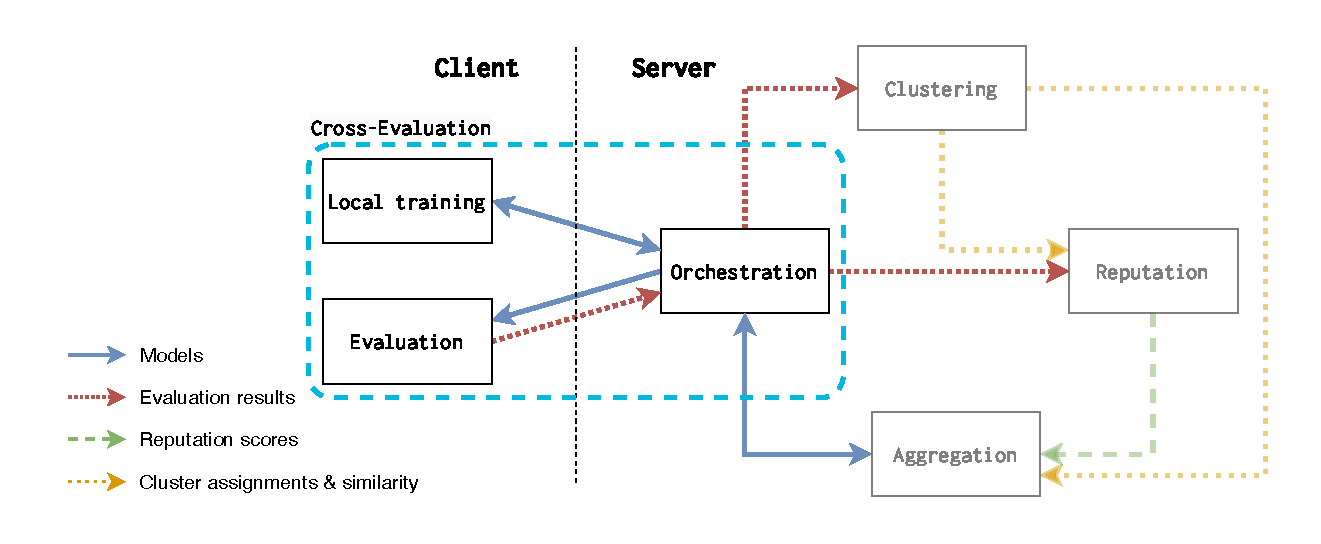
\includegraphics[width=\textwidth]{figures/radar-xeval.pdf}
        };
        
        \node[align=left, anchor=north west] at (.05,.91) {\begin{minipage}{.7\textwidth}\subsectionpage\end{minipage}};
    }
\end{frame}

\begin{frame}{Assessing Quality with Cross-Evaluation}

  \begin{columns}
    \begin{column}{.45\textwidth}
      \begin{figure}
        \centering
        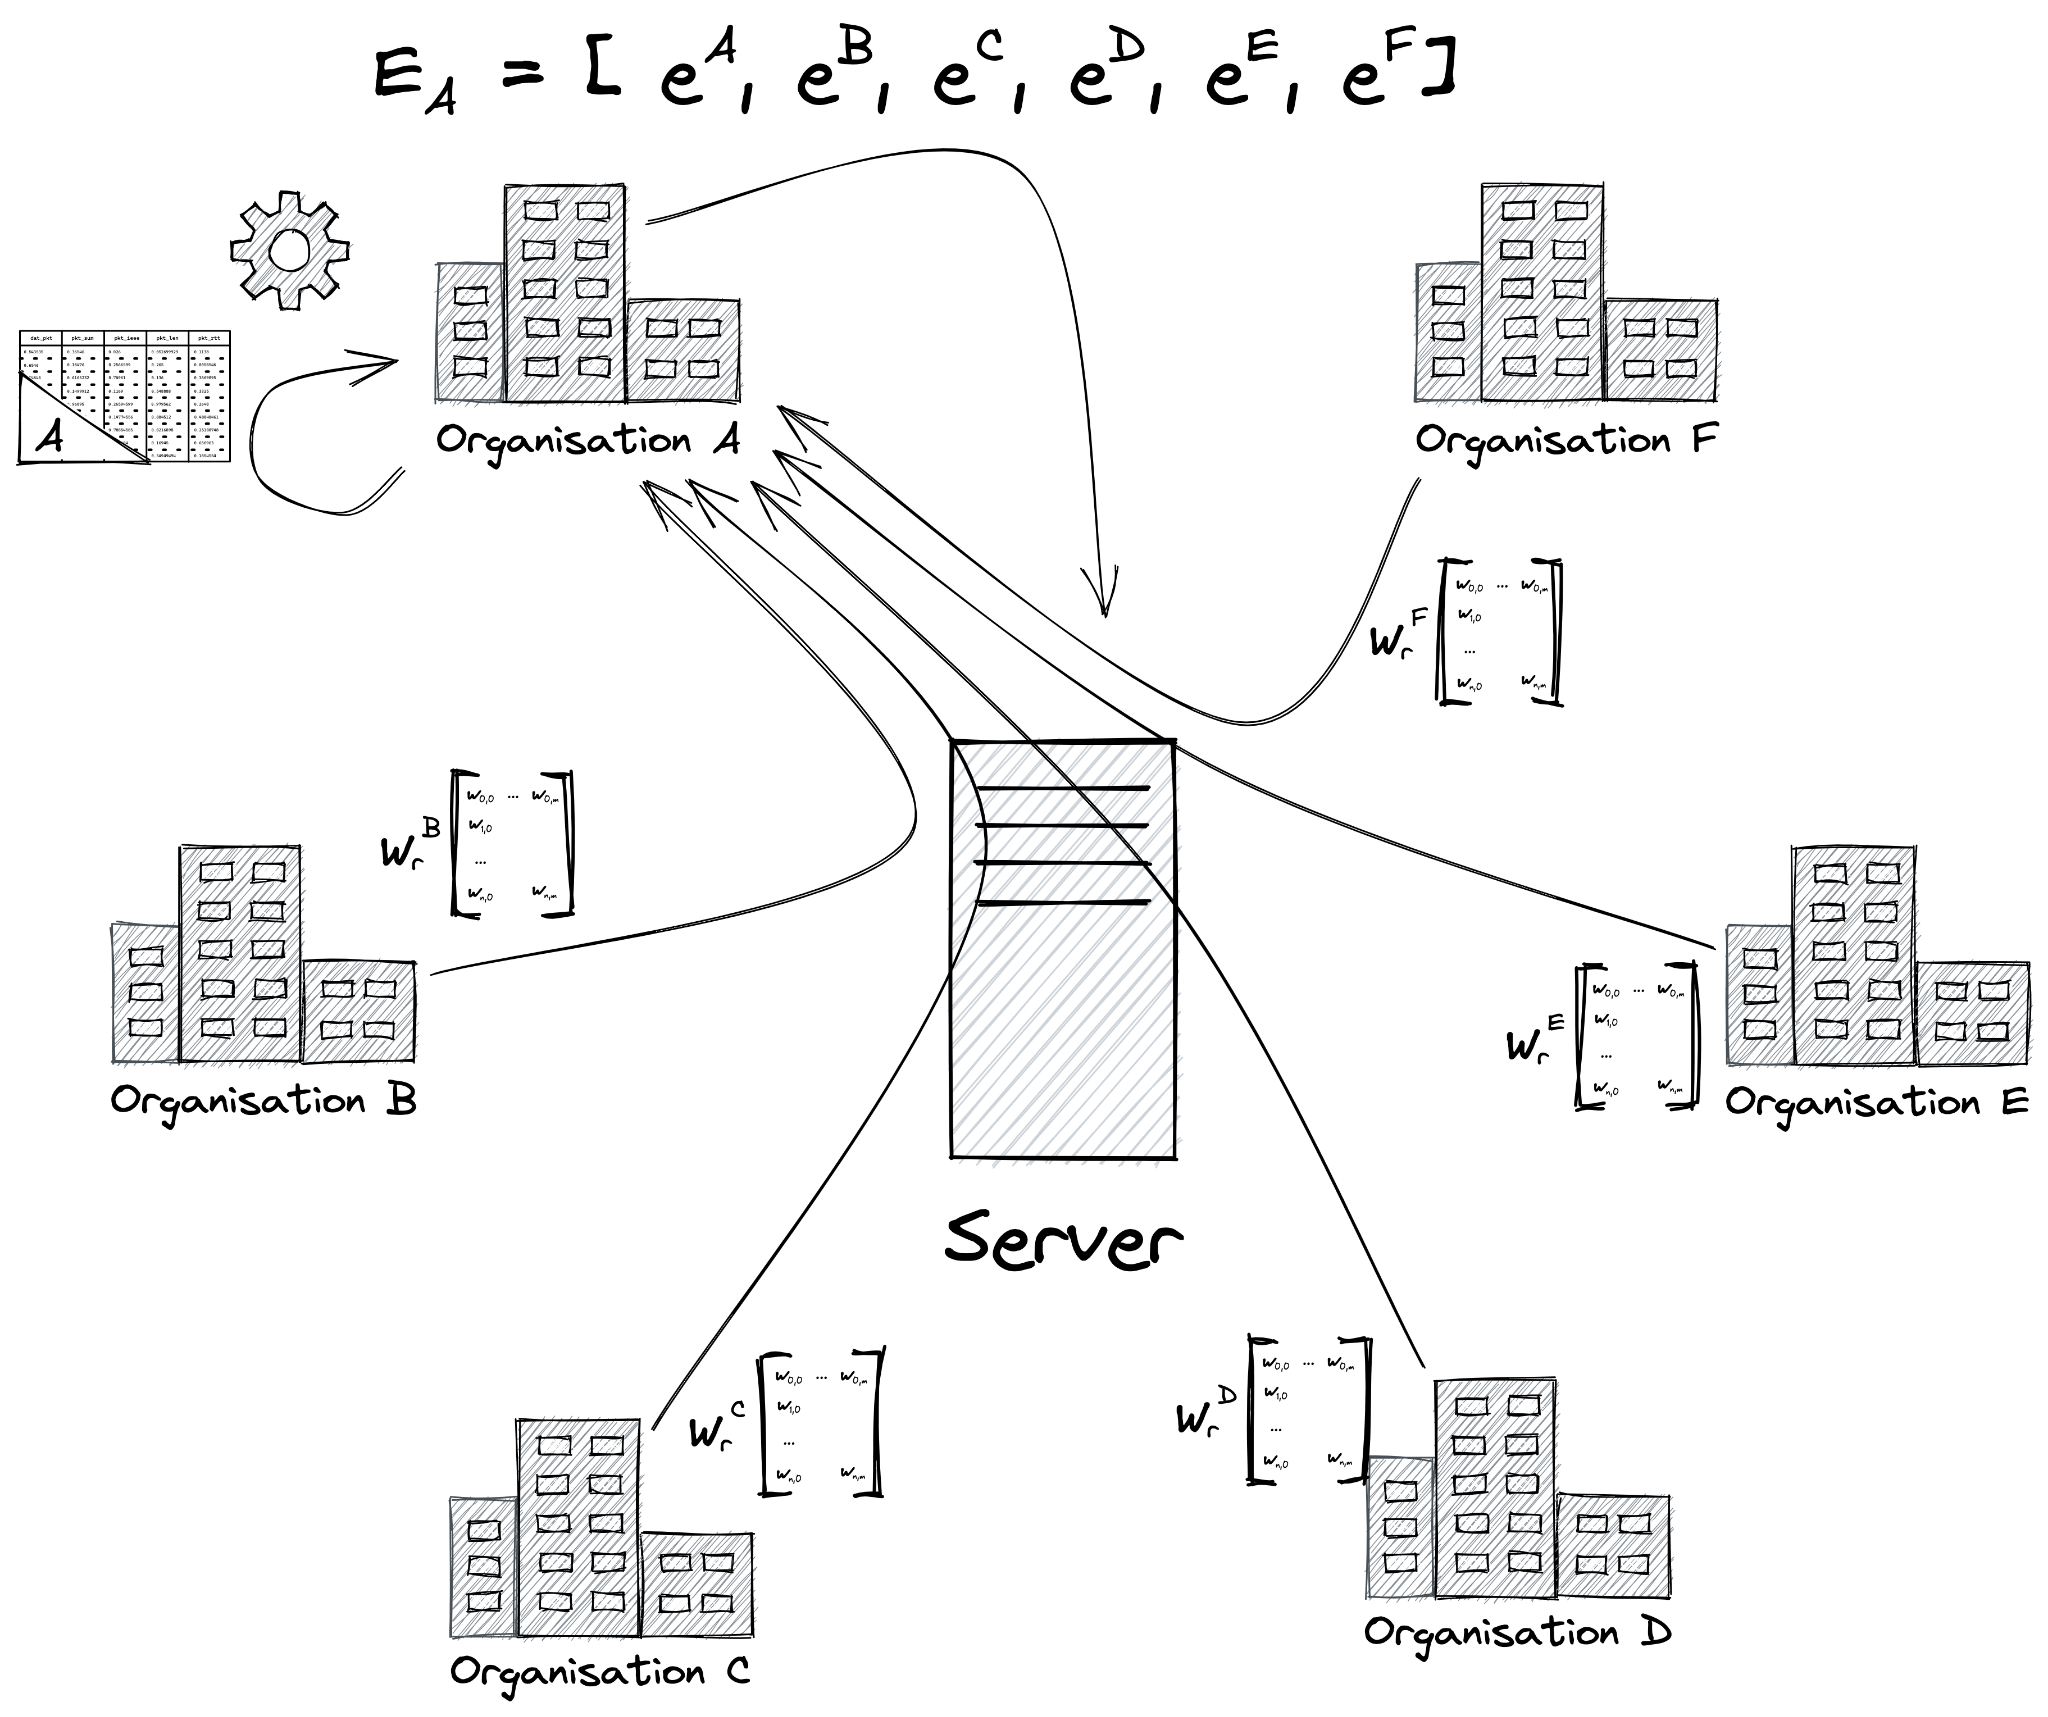
\includegraphics[width=\textwidth]{figures/radar/xeval}
      \end{figure}
    \end{column}
    
    \begin{column}{.55\textwidth}
      \small
      \setlength{\baselineskip}{0.8\baselineskip}
      \vspace{1ex}

      \textbf{Advantages}
      \begin{itemize}
        \item The central server does not need prior knowledge.
        \item Evaluates how each model fits the data (\eg, accuracy, F1 score).
        \item Exhaustive overview of the entire system at each round $r$.
      \end{itemize}

      \pause
      \textbf{Drawbacks}
      \begin{itemize}
        \item High communication and computation costs.
        \item Does not scale well.
        % \item Shares local models to participants: less privacy-friendly.
      \end{itemize}


      \pause
      \textbf{But\dots}
      \begin{itemize}
        \item Cross-silo use case: few clients, with reasonable computing capacity.
        \item Slow workflow: long time between rounds.
      \end{itemize}
    \end{column}

  \end{columns}

\end{frame}

\subsection{Fighting Heterogeneity with Clustering}
% Discours à porter sur cette slide  : 
% Build \emph{more} homogeneous communities of participants to facilitate model aggregation.
% 1 different model per more homogeneous community.
% X-eval results not models : as explained earlier evaluations are representative of participants data distribution. 
\begin{frame}
    \tikz[overlay, remember picture,
      shift=(current page.south west),
      x=(current page.south east),
      y=(current page.north west)
    ]{      
        \node[anchor=south east] at (1,0) {
            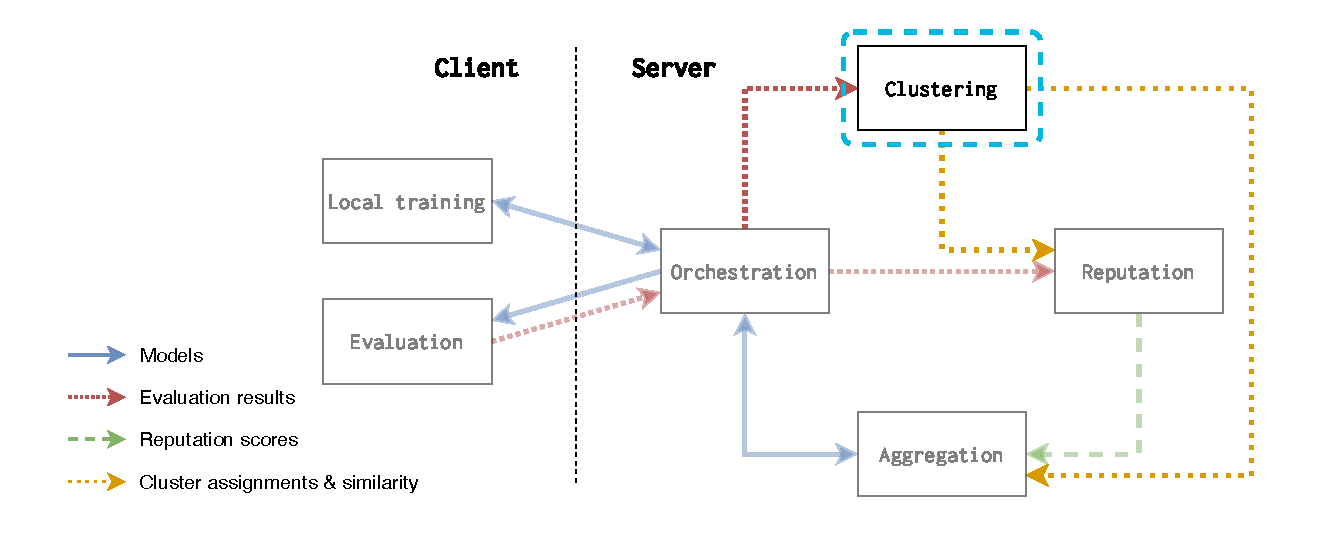
\includegraphics[width=\textwidth]{figures/radar-clust.pdf}
        };
        
        \node[align=left, anchor=north west] at (.05,.91) {\begin{minipage}{.7\textwidth}\subsectionpage\end{minipage}};
    }
\end{frame}
% \begin{frame}{Fighting Heterogeneity with Clustering}
%   % Un ptit graph içi ça ne mangerait pas de pain. 
%   \textbf{Objective}
%   \begin{itemize}
%     \item Build \emph{more} homogeneous communities of participants to facilitate model aggregation.
%   \end{itemize}


%     \pause
%     \textbf{Clustering for FL}\\
%     Leverage cross-evaluation results instead of model updates:
%         \begin{itemize}
%             \item subjective similarity estimation;
%             \item similar evaluations $\rightarrow$ similar data distributions;
%         \end{itemize}
% \end{frame}

\begin{frame}{Fighting Heterogeneity with Clustering}
%Discours :
% Cosine sim : angle measure that will reflect even small changes in a single parameter. 
% Parler du thresold dynamique et de sa méthode de calcul. 
% Exemple rapide du hierarchical clustering.
    \begin{columns}
        \begin{column}{.5\textwidth}
        \begin{itemize}
                \item Distance metric
                \begin{itemize}
                    % \item Between models/gradients;
                    \item Based on \alert{cross-evaluation} results. 
                    \item \alert{Cosine similarity}~\cite{briggs_Federatedlearninghierarchical_2020}.
                \end{itemize}
        \end{itemize}
        \onslide<2->{
            \begin{itemize}
                \item Algorithm
                \begin{itemize}
                    % \item Dynamic \emph{split-and-merge}.~\autocite{chen_ZeroKnowledgeClustering_2021}
                    \item \alert{Hierarchical clustering}.~\autocite{briggs_Federatedlearninghierarchical_2020}
                    \item Dynamic aggregation threshold. 
                \end{itemize}
                \end{itemize}
        }
        \end{column}
        \onslide<3->{
        \begin{column}{.5\textwidth}
            \begin{figure}
                \centering
                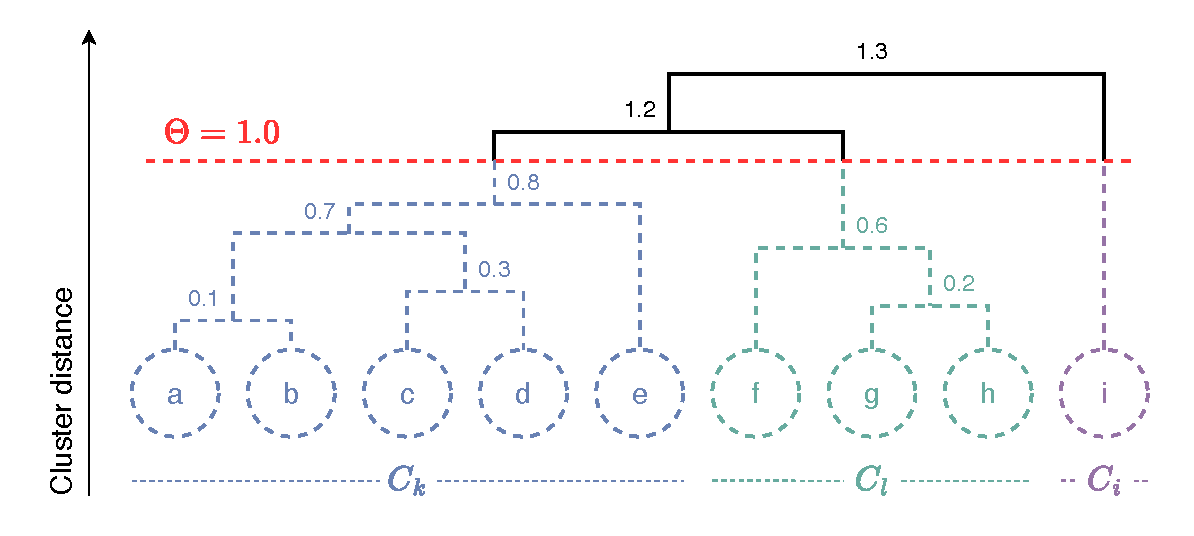
\includegraphics[width=\textwidth]{figures/radar/clustering.drawio.pdf}
                % \makebox[\textwidth][c]{%
                %   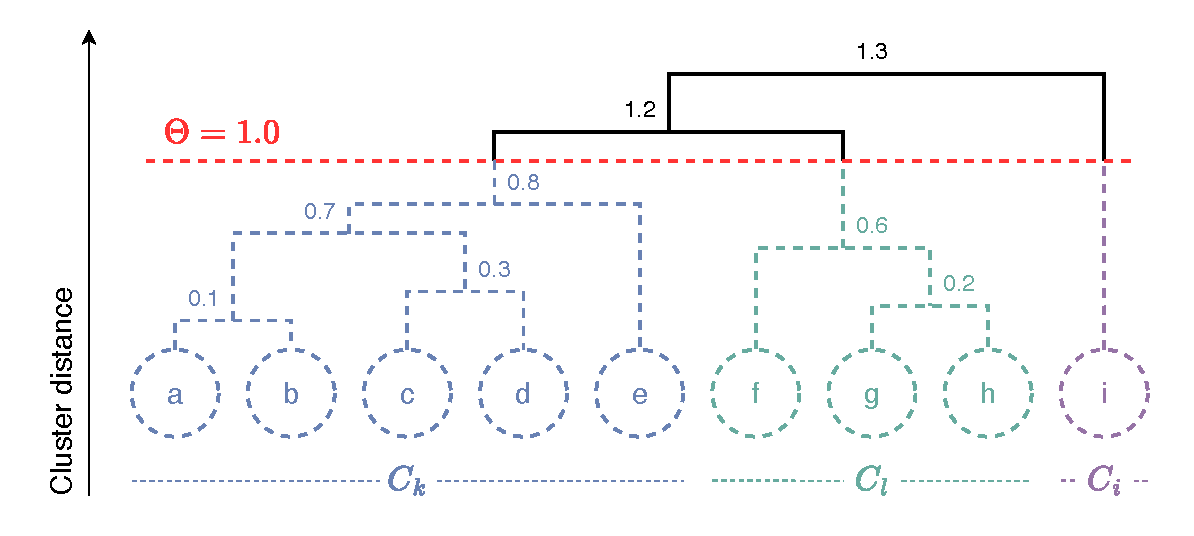
\includegraphics[width=1.2\textwidth]{figures/radar/clustering.drawio.pdf}%
                % }
                \caption{Hierarchical clustering.}
            \end{figure}
        \end{column}
        }
    \end{columns}
    % \only<2->
    \fcitefootnote{briggs_Federatedlearninghierarchical_2020}
    % \fcitefootnote{chen_ZeroKnowledgeClustering_2021}
\end{frame}



\subsection{Mitigating Byzantine Contributions}

\begin{frame}
    \tikz[overlay, remember picture,
      shift=(current page.south west),
      x=(current page.south east),
      y=(current page.north west)
    ]{
        \node[anchor=south east] at (1,0) {
            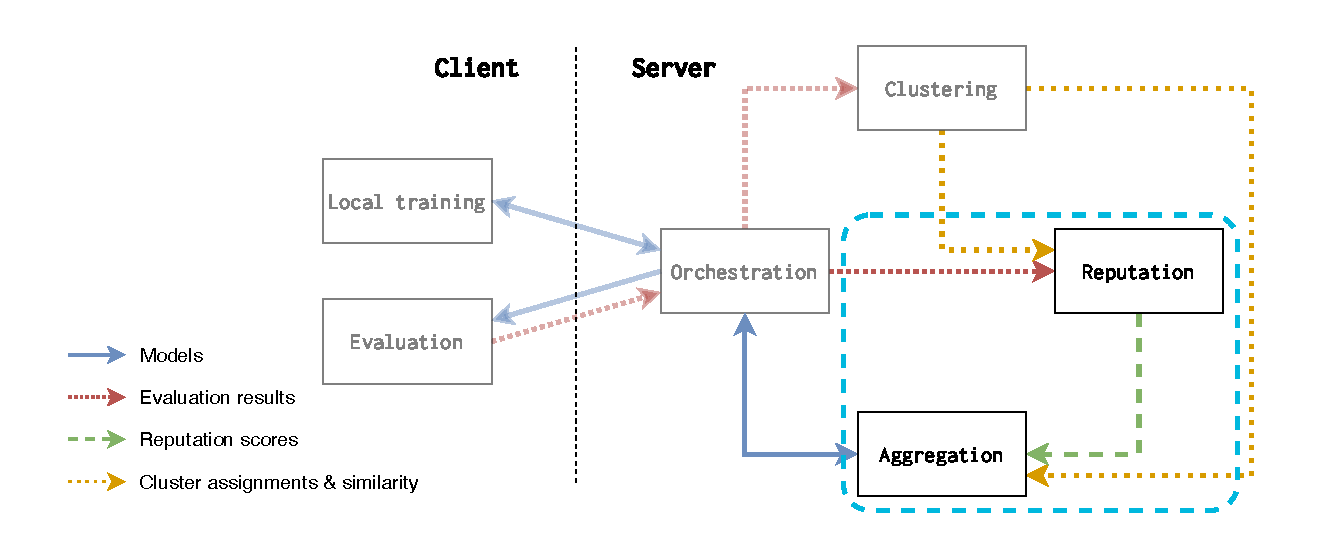
\includegraphics[width=\textwidth]{figures/radar-reput.pdf}
        };
        
        \node[align=left, anchor=north west] at (.05,.91) {\begin{minipage}{.7\textwidth}\subsectionpage\end{minipage}};
    }
\end{frame}
\begin{frame}{Reputation-aware Aggregation}
% Point de discours 
% Déf + pq ça match pour nous.
% On fait de la pondération de modèles plus pertinent pour nous que du choix de modèles.
  \begin{block}{Definition: Reputation Systems
    \begingroup            \color{white}\normalfont~\autocite{resnick_Reputationsystems_2000}}.
    \endgroup
    \begin{itemize}
      \item Long-lived entities that inspire an expectation of future interaction;
      \item Capture and distribution of feedback about current interactions (such information must be visible in the future); and
      \item Use of feedback to guide trust decisions.
    \end{itemize}
  \end{block}

  \onslide<2>{%
    \begin{itemize}
      % \item Dirichlet distribution for local aggregation of the reputation scores.~\autocite{fung_DirichletBasedTrustManagement_2011}
      % \item Votes weighted by the similarity inside each cluster.
      \item Votes weighted based on their similarity to other cluster members. 
      \item Exponential decay to track behavior over time.
    \end{itemize}
  }

  \fcitefootnote{resnick_Reputationsystems_2000}
  % \only<2>{%
  %   \fcitefootnote{fung_DirichletBasedTrustManagement_2011}
  % }

\end{frame}

